\documentclass[11pt,a4paper]{report}
%\usepackage[T1]{fontenc}
%\usepackage[english]{babel}
%\usepackage[latin1]{inputenc}
\includeonly{c_bording, n_lawrance}
\includeonly{e_hackett}
\includeonly{l_salter2}
%,j_tapley,n_lawrance,l_salter,i_gao,l_scarlett,e_perica,a_sorbello,i_lau,j_panggalo,c_norman,o_erkilic,e_thgesen,e_hackett,n_lawler,e_raptakis,r_mapondera}

\title{The Pawsey Summer Internship Cookbook}
\author{C.Bording, J.Tapley, N.Lawrance,\\
L.Salter, I.Gao, L.Scarlett, E.Perica,\\
A.Sorbello, I.Lau, J.Panggalo, C.Norman,\\
O.Erkilic, E.Thgesen, E.Hackett,\\
N.Lawler, E.Raptakis, R.Mapondera}

\begin{document}
\maketitle
\tableofcontents


\begin{abstract}

This is a simple project to help the Pawsey Supercomputing Centre summer intership students re-enforce their understanding of \TeX and use of Git with github!

\end{abstract}

\chapter{Chris Bording}
\section{My Biography}
Chris Bording biography for the Pawsey Supercomputing Centre Summer internship
\subsection{about me!}
I am a Senior Supercomputing Specialist, with a background in Scientific Computing and Mechanical Engineering.I specialize in Fortran/C/C++ with MPI applications.  I am hoping to develop my programming skills this using the Intel Knights Corner and Knights Landing systems.  I have the great priviledge of being in charge of the 
Pawsey Supercomputing Summer Internship program this year!



<<<<<<< HEAD
=======
\chapter{Nicholas Lawrance}
\section{Nicholas Lawrance}

Nicholas studied a Bachelor of Philosophy with a double major in mathematics and computer science at UWA and completed his honours year in applied maths with a topic in network science looking at the Perth water network. For his Pawsey project he will be parallelising existing network analysis algorithms to allow larger networks to be studied. He will then use these algorithms to characterise large networks that would otherwise have been infeasible. This project is partially motivated by his honours project where he encountered significant computational boundaries due to the network's size, it contained 240,000 nodes and 267,000 links. Now that he has completed his degree, Nicholas plans to work in data analysis making use of his maths and computing skills. 



\chapter{Emily Hackett}
\section{Chocolate Chip Cookies}

\section{Ingredients}
\begin{itemize}
\item 3/4 cup granulated sugar
\item 3/4 cup packed brown sugar
\item 1 cup butter or margarine, softened
\item 1 teaspoon vanilla
\item 1 egg
\item 2 1/4 cups all-purpose flour
\item 1 teaspoon baking soda
\item 1/2 teaspoon salt
\item 1 cup coarsely chopped nuts
\item 1 package (12 ounces) chocolate chips (2 cups)
\end{itemize}

\section{Instructions}
\begin{enumerate}
\item  Heat oven to 375ºF.
\item Mix sugars, butter, vanilla and egg in large bowl. Stir in flour, baking soda and salt (dough will be stiff). Stir in nuts and chocolate chips.
\item Drop dough by rounded tablespoonfuls about 2 inches apart onto ungreased cookie sheet.
\item Bake 8 to 10 minutes or until light brown (centers will be soft). Cool slightly; remove from cookie sheet. Cool on wire rack.
\end{enumerate}

\section*{Expert Tips}
Can also try with 1/2 cup each of peanut butter chips, or dark chocolate chips or butterscotch chips.




\chapter{Liam Salter}
\section{Shortbread}

\begin{itemize}
	\item 125g/4oz butter
	\item 55g/2oz caster sugar, plus extra to finish
	\item 180g/6oz plain flour
\end{itemize}

\subsection{Method}

\begin{enumerate}
\item Heat the oven to 190C/375F/Gas 5.
\item Beat the butter and the sugar together until smooth.
\item Stir in the flour to get a smooth paste. Turn on to a work surface and gently roll out until the paste is 1cm/in thick.
\item Cut into rounds or fingers and place onto a baking tray. Sprinkle with caster sugar and chill in the fridge for 20 minutes.
\item Bake in the oven for 15-20 minutes, or until pale golden-brown. Set aside to cool on a wire rack.
\end{enumerate}

\begin{figure}[h]
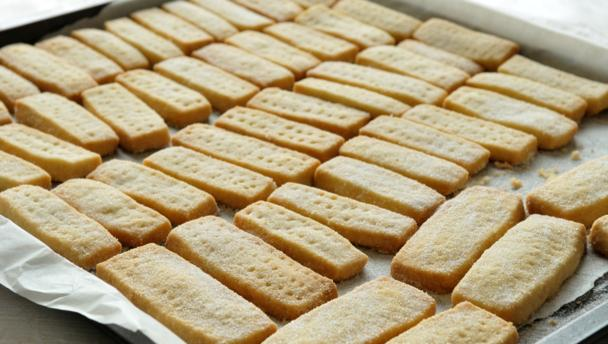
\includegraphics[width=8cm]{shortbread}
\caption{this is a picture of shortbread}
\end{figure}


\chapter{Liam Scarlett}
\section{Spinach, feta and broad bean pie}
This fabulous vegetarian pie contains broad beans, fetta cheese and spinach in a crunchy wholemeal pastry.
\section{Ingredients:}
\begin{itemize}
	\item 2 cups wholemeal plain flour
	\item 1 cup wheatgerm
	\item 160g butter, chilled, chopped
	\item 4 eggs
	\item 2 tablespoons chilled water
	\item 2 teaspoons olive oil
	\item 1 large brown onion, finely chopped
	\item 2 garlic cloves, crushed
	\item 200g baby spinach
	\item 2 cups (300g) fresh broad beans
	\item 100g feta, crumbed
	\item 2 tablespoons finely grates hard cheese or parmesan
	\item 1 tablespoon chopped fresh dill
	\item 1 teaspoon finely grated lemon rind
	\item 1/3 cup milk
\end{itemize}

\section{Instructions:}
\begin{enumerate}
\item Place flour, wheatgerm and butter in a food processor. Process until mixture resembles fine breadcrumbs. Add 1 egg and chilled water. Process until mixture just comes together and forms a soft dough, adding extra water if necessary. Turn out onto a lightly floured surface. Knead until smooth. Shape into a disc. Wrap in plastic wrap. Refrigerate 30 minutes or until firm.
\item Meanwhile, heat oil in a large, deep frying pan over medium-high heat. Add onion. Cook for 5 minutes or until softened. Add garlic. Cook, stirring, for 1 minute or until fragrant. Add spinach. Cook for 2 minutes or until wilted. Transfer mixture to a colander over a bowl to strain. Cool for 10 minutes.
\item Place broad beans in a heatproof bowl. Cover with boiling water. Set aside for 30 seconds. Drain. Refresh in a bowl of chilled water. Drain. Peel and discard skins.
\item Preheat oven to 190C/170C fan-forced. Roll pastry out between 2 sheets of baking paper until 5mm thick. Line a 4cm-deep, 22cm (top) pie plate with pastry. Trim excess. Pinch edge of pastry to form a decorative pattern.
\item Place spinach mixture in a bowl. Add broad beans, fetta, cheese, dill and lemon rind. Whisk milk and remaining eggs together. Add to broad bean mixture. Season with salt and pepper. Stir until well combined. Spoon mixture into pastry case. Place on a baking tray. Bake for 45 minutes or until golden and filling has set. Stand for 10 minutes. Cut into wedges. Serve.
\end{enumerate}


\chapter{Ivan Lau}
\section{My Biography}
Ivan Lau biography for the Pawsey Supercomputing Centre Summer Internship

\subsection{About Me}
I am a third year Medical Imaging student from Curtin University and just about to enter my exciting final year next year. The project that I will be working on in this internship will be about determining the clinical value of realistic 3D printed heart models in helping physicians to understand patient-specific cardiovascular pathology and thus improving the presurgical planning in congenital heart diseases. 
I am hoping to gain experience and develop skills in planning and conducting scientific and academic research, and more importantly, I am excited to see how the programming skills and supercomputers can help me to conduct a much better and faster research.




>>>>>>> b4f9433f767a85e510d13dfe03f2adb6434721af
\end{document}

